\documentclass[a4paper, 10pt]{article}

\usepackage[utf8x]{inputenc}
\usepackage[english, russian, ukrainian]{babel}
\usepackage{cmap}
\usepackage{mathtext}
\usepackage[T2A]{fontenc}

\usepackage{graphicx}
\usepackage{float}
\usepackage{listings}

\usepackage{geometry}
\geometry{top = 2cm}
\geometry{bottom = 2cm}
\geometry{left = 3cm}
\geometry{right = 1.5cm}

\begin{document}
\begin{titlepage}
\begin{center}
\large{
Міністерство освіти і науки, молоді та спорту України\\
Національний технічний університет України\\
``Київський політехнічний інститут''\\
Факультет прикладної математики\\
Кафедра спеціалізованих комп’ютерних систем\\
}

\vfill

\large{\bf{
Лабораторна робота №4\\
Дисципліна:\\
``Архітектура комп'ютерів''\\
Тема:\\
``Програмування циклів і умовних переходів''\\
}}

\vfill

\begin{table}[h]
\centering
\begin{tabular}{lp{4cm}l}
Виконав:&&Перевірив:\\
Студент групи КВ--92&&Жабін В. І.\\
Гуль О. В.&&\\
Залікова книжка № КВ--9203&&\\
\end{tabular}
\end{table}

\vfill

Київ \the\year
\end{center}
\end{titlepage}
\newpage

\section{Мета}
Вивчити принципи програмування циклів і умовних переходів з використанням команд управління і з урахуванням специфіки виконання програм на ОС під управлінням потока даних.

\section{Завдання}
\begin{enumerate}
    \item Вивчити ОС з буферною пам'яттю даних і з асоціативною пам'яттю. При вивченні звернути увагу на формат даних і специфіку програмування. Так само при вивченні ОС з буферною пам'яттю даних звернути увагу на алгоритми опиту буферної пам'яті.
    \item Визначити 7 молодших розрядів двійкового представлення номера залікової книжки.
    \item Згідно цим цифрам визначити свій варіант лабораторної роботи.
    \item Побудувати програму для ВС, використовуючи графічне відображення команд.
    \item Виконати адресацію всіх операцій.
    \item Написати програму виконання заданої функції.
\end{enumerate}

\noindent
Варіант: $9203=10001111110011_2.$\\
$a_{6},\cdots,a_{0}=1110011.$\\
\begin{lstlisting}[numbers=left, language=pascal]
F:=1;
For i:=2 to n  do
    F:=f*i;           {f=n!}
\end{lstlisting}
$N = 5.$\\
Виведення на пристрій: $4.$\\
Примітка: Для всіх варіантів кількість пристроїв виводу~-- 4.\\

\section{Порядок виконання роботи}
\begin{enumerate}
    \item Набрати в редакторі програму. Запустити її на виконання і перевірити правильність виконання функції. У разі потреби можна знайти помилки, використовуючи відладчик.
    \item Представити викладачеві результати виконаної роботи.
	\item Зробити висновки по роботі.
\end{enumerate}

\section{Виконання завдання}
\begin{figure}[H]
\begin{center}
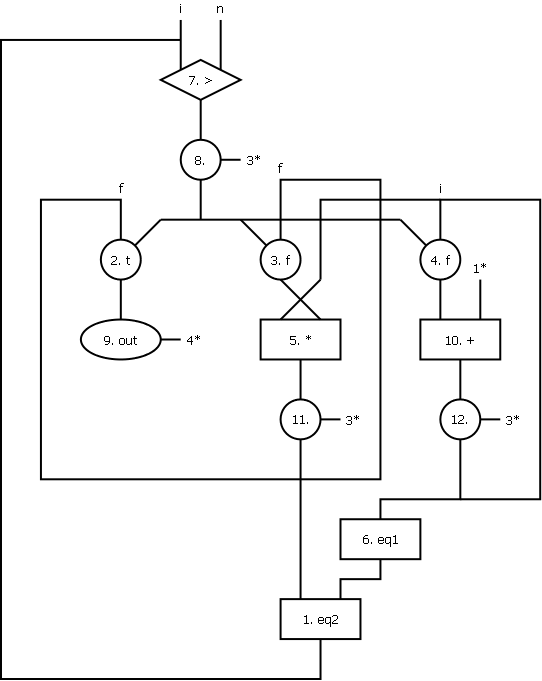
\includegraphics[scale=0.5, angle=90]{lab4_alg.png}
\caption{Граф програми обчислення.}
\end{center}
\end{figure}

\begin{figure}[H]
\begin{center}
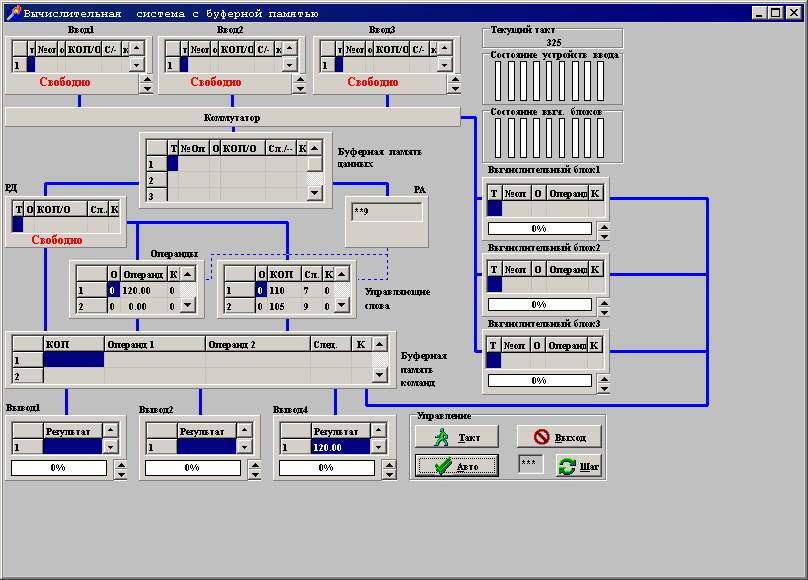
\includegraphics[scale=0.75]{lab4.png}
\caption{Результат виконання.}
\end{center}
\end{figure}

lab4.asm
\begin{lstlisting}[numbers=left]
program lab4
constant
i = 2
n = 5
f = 1
begin
 1: eq2   0*,  _, !0 to  7
 2: if     f,  _, !0 to  9
 3: ifnot  f,  _, !1 to  5
 4: ifnot  i,  _, !0 to 10
 5: mul    i,  _, !0 to 11
 6: eq1    _, 0*, !1 to  1
 7: cmpm   i, n*, !0 to  8
 8: xn     _, 3*, !1 to  2
 9: out    _, 4*, !0 to  9
10: add    _, 1*, !0 to 12
11: xn     _, 3*, !0 to  1
12: xn     _, 3*, !0 to  4
end
\end{lstlisting}

Результат отриманий для:\\
\begin{itemize}
	\item Кількість пристроїв введення: 6.
	\item Кількість пристроїв виведення: 4.
	\item Кількість процесорів: 16.
	\item Довжина буферної пам'яті даних: 16.
	\item Довжина буферної пам'яті команд: 16.
	\item Розмір пам'яті: 128.
	\item Параметри часу виконання команд~-- стандартні.
	\item Алгоритм опитування: з вільною коміркою БПД.
	\item Система: з буферною пам'яттю.
\end{itemize}

\section{Висновки}
Програмування логічних умов, переходів та циклів суттєво відрізняється у ОС, що керуються потоком даних та таких, що керуються потоком команд.
\end{document}
